\newcommand{\latex}{\LaTeX~}
\newcommand{\latexx}{\LaTeX}

\chapter{\latex}

Bu bölümde, \latex tanıtılacak ve hakkında genel kültür bilgileri verilecektir.

\section{\latex Nedir?}
\latexx; makale, kitap, tez, sunum, poster gibi özellikle bilimsel çalışmaların yazılmasında ve raporlamasında kullanılan doküman hazırlama sistemidir. Bilim dünyasında neredeyse standart haline gelmiş \latexx'in yüksek kalitede çıktılar üretmesi, üretilen çıktıların farklı sürüm ve platformlarda kaymalara ve dağılmalara sebep olmaması, ücretsiz olması, derlenebilir bir dil olduğundan şarta bağlı ifadelerin rahatlıkla kullanılabilmesi, sayfa hakimiyetinin tamamen kullanıcıda olması vs. gibi pek çok avantajı vardır.

\section{\latex Nasıl Okunur?}
\latexx; ilk defa kullanmaya başlayan ya da \latex kullanıcısı olmayan birçok insan tarafından genelde \textit{la-teks} veya \textit{ley-teks} şeklinde okunur. \latex kelimesinin İngilizce bir kelime olduğu düşüncesiyle bu şekilde okunmaktadır. İngilizcede \textit{latex} diye bir kelime vardır ve \textit{ley-teks} diye okunur ancak bu kelime kauçuk ağacından çıkarılmış maddeyi ifade etmektedir. 

\TeX~ kelimesi Yunan alfabesinde \textbf{tau}, \textbf{epsilon} ve \textbf{chi} harflerinden meydana gelmiştir. Buradaki \textbf{chi} harfi  \textit{Ki} şeklinde okunmaktadır. Bundan ötürü \latex kelimesi okunurken \textit{lah-tek} veya \textit{ley-tek} şeklinde okunur. 

\section{\latex mi, Word mü?}
Word varken niçin \latex kullanalım?, sorusu birçok Word kullanıcısının sorduğu ilk sorudur? Word tarzı belge düzenleme programları WYSIWYG (What You See Is What You Get/Ne Görürsen Onu Alırsın) adı altında toplanmaktadırlar. Bu ifade belgeyi oluştururken belgenin son haline en yakın halinin görülerek hazırlanmasından kaynaklanmaktadır. Ancak \latex belgeleri yazılırken dokümanın nihai hali belge oluşturulurken görülmemektedir.

\begin{figure}[!ht]
  \centering
  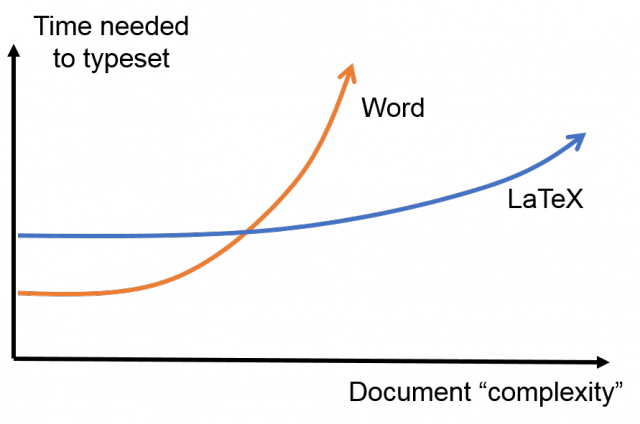
\includegraphics[width=0.6\textwidth]{zkilavuz/wordvslatex}
  \caption{Word ve \latex belgeleri hazırlanırken belge karmaşıklığına göre harcanan zaman grafiği}
  \label{fig:wordvslatex}
\end{figure}

\latex mi, Word mü? sorusu ile ilgili birçok çalışma yapılmıştır \cite{knauff2014efficiency, brischoux2009don}. Bu çalışmalar sonucunda Şekil-\ref{fig:wordvslatex} bu çalışmalar sonucu elde edilmiş bir grafiği göstermektedir. Kullanıcılar üzerinde yapılan çeşitli deneyler sonucunda dokümanın karmaşıklığı arttıkça \latex kullanmanın daha verimli olduğu gösterilmiştir.

\begin{table}[!ht]
\centering
\caption{Word ile \latexx'in çeşitli kriterlere göre 3 puan üzerinden değerlendirilmesi}
\label{table:wordvslatex}
\begin{tabular}{|c|c|c|}
\hline
\textbf{Özellik}                                                                               & \textbf{Word Puanı} & \textbf{Latex Puanı} \\ \hline
Küçük doküman hazırlama hızı                                                                   & 3                   & 2                    \\ \hline
\begin{tabular}[c]{@{}c@{}}Büyük doküman hazırlama ve \\ grafiklerle uğraşma hızı\end{tabular} & 1                   & 3                    \\ \hline
Kullanma kolaylığı                                                                             & 3                   & 1                    \\ \hline
Düzen ve çıktı kalitesi                                                                        & 2                   & 3                    \\ \hline
Bilimsel özellikler                                                                            & 1                   & 3                    \\ \hline
Ücret ve kullanılabilirlik (erişilebilirlik)                                                   & 1                   & 3                    \\ \hline
Uyumluluk                                                                                      & 2                   & 2                    \\ \hline
\textbf{Toplam}                                                                                & \textbf{13}         & \textbf{18}          \\ \hline
\end{tabular}
\end{table}

Tablo-\ref{table:wordvslatex},  çeşitli kriterlere göre Word ve \latex kullanmanın puanlamasını göstermektedir. 

\latexx'in Word'e göre kesin olan bazı avantajlarını şu şekilde sıralayabiliriz:

\begin{itemize}
    \item Yazılan belgeler herhangi bir editör ile okunabilir veya yazılabilir. Genellikle \texttt{.txt} editörleri yazıları görmek için yeterlidir. Ancak Word için Office Word programının yüklü olması gerekmektedir.
    \item \latex çıktı olarak (kullanıcının isteğine bağlı olarak) PDF üretir. Haliyle çıktılar farklı ortamlarda kaymalara, bozukluklara sebep olmaz. 
    \item Word belgeleri hazırlanırken oluşan düzen bozuklukları, dokümanı oluştururken aksamalara veya vakit kaybına sebep olabilmektedir. \latex kullanıcıları dokümanı hazırlarken tamamen belgenin içeriğine odaklanırlar.
    \item Word belgelerinde kopyalama işlemi çoğu zaman problemlere yol açmaktadır. Farklı bir belgeye kopyalandığında o belgenin düzenine uydurulması, düzenlenmesi gerekmektedir. Ancak \latex için kopyalama çok kolaydır. Sitil dosyası farklı olduğundan, sitil dosyası değiştiğinde düzen otomatik olarak değişir ve kullanıcı farklı belgeler için aynı dosyayı düzenlemekle uğraşmaz.
    \item Düzen, yazı tipleri, tablolar, şekiller vs. hepsi hazırlanan doküman boyunca tutarlıdır.
    \item Dizinler, dipnotlar, alıntılar, kaynaklar, içindekiler vs. kolaylıkla üretilebilir.
    \item Matematiksel formüllerin metin içerisindeki kalitesi yüksektir.
\end{itemize}

Elbetteki \latex için de bazı olumsuzluklar var. Örneğin yazılan dokümanın son halini yazıyı yazarken görememek (Word kullanmadan gelen alışkanlık) kullanıcılarda başlangıçta tedirginliğe sebep olmaktadır. Ancak zamanla alışılan bir durumdur. Eğer dokümanı siz biçimlendirmek istiyorsanız biçimlendirme komutlarını bilmeniz gerekmektedir. 

Şekil-\ref{fig:ornekgrafik} \latex kullanılarak çizilmiştir. Word kullanarak çizmenin çok zor olduğu bu ve benzeri şekiller basit ve kısa kodlarla çok rahat bir biçimde yapılabilmektedir. Bu şekli çizen kod aşağıda verilmiştir (\textbf{Not:} \latexx'de karmaşık şekil çizimleri profesyonellik gerektirmektedir. İleri seviyede olmayanlar için bu kodlar karmaşık gelebilir. Tez yazımında bu profesyonellik beklenmemektedir. )

\begin{minted}{latex}
\tikzstyle{every node}=[circle, draw, fill=black!50,
                        inner sep=0pt, minimum width=4pt]
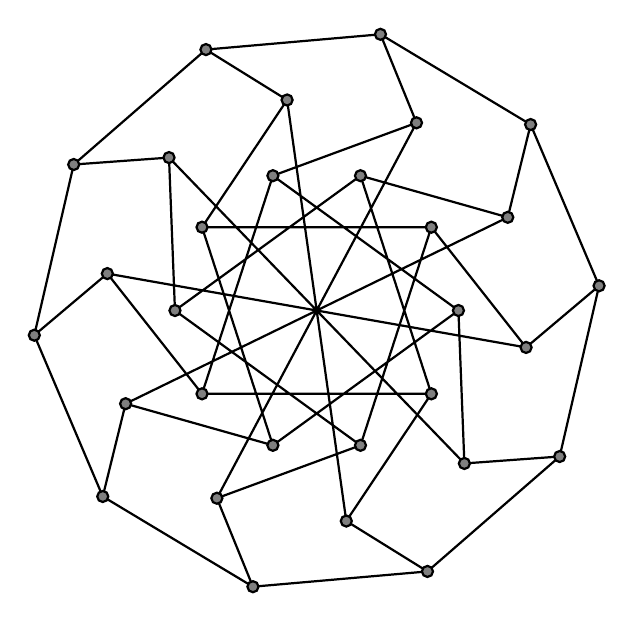
\begin{tikzpicture}[thick,scale=0.9]
    \draw \foreach \x in {0,36,...,324}
    {
        (\x:2) node {}  -- (\x+108:2)
        (\x-10:3) node {} -- (\x+5:4)
        (\x-10:3) -- (\x+36:2)
        (\x-10:3) --(\x+170:3)
        (\x+5:4) node {} -- (\x+41:4)
    };
\end{tikzpicture}
\end{minted}

\begin{figure}[!ht]
  \centering
\tikzstyle{every node}=[circle, draw, fill=black!50,
                        inner sep=0pt, minimum width=4pt]
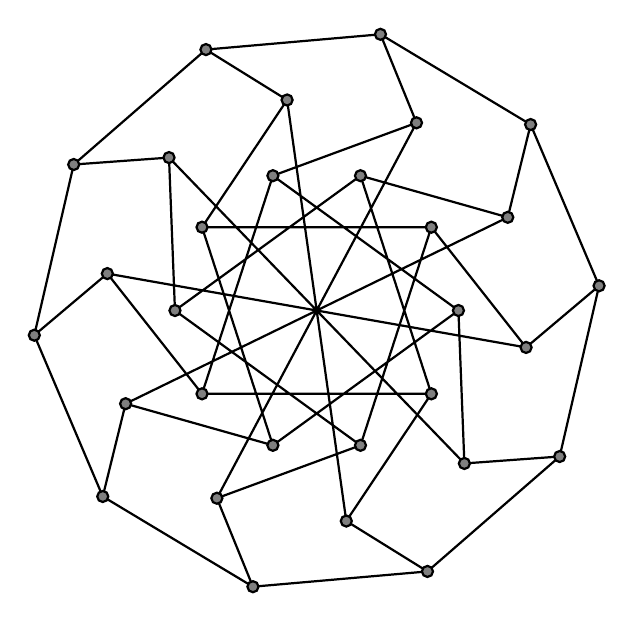
\begin{tikzpicture}[thick,scale=0.9]
    \draw \foreach \x in {0,36,...,324}
    {
        (\x:2) node {}  -- (\x+108:2)
        (\x-10:3) node {} -- (\x+5:4)
        (\x-10:3) -- (\x+36:2)
        (\x-10:3) --(\x+170:3)
        (\x+5:4) node {} -- (\x+41:4)
    };
\end{tikzpicture}
  \caption{\latex ile çizilmiş örnek bir şekil}
  \label{fig:ornekgrafik}
\end{figure}

\begin{figure}[!ht]
  \centering
\usetikzlibrary{lindenmayersystems}
\usetikzlibrary[shadings]
\pgfdeclarelindenmayersystem{Fractal plant}{
  \rule{X -> F-[[X]+X]+F[+FX]-X}
  \rule{F -> FF}}
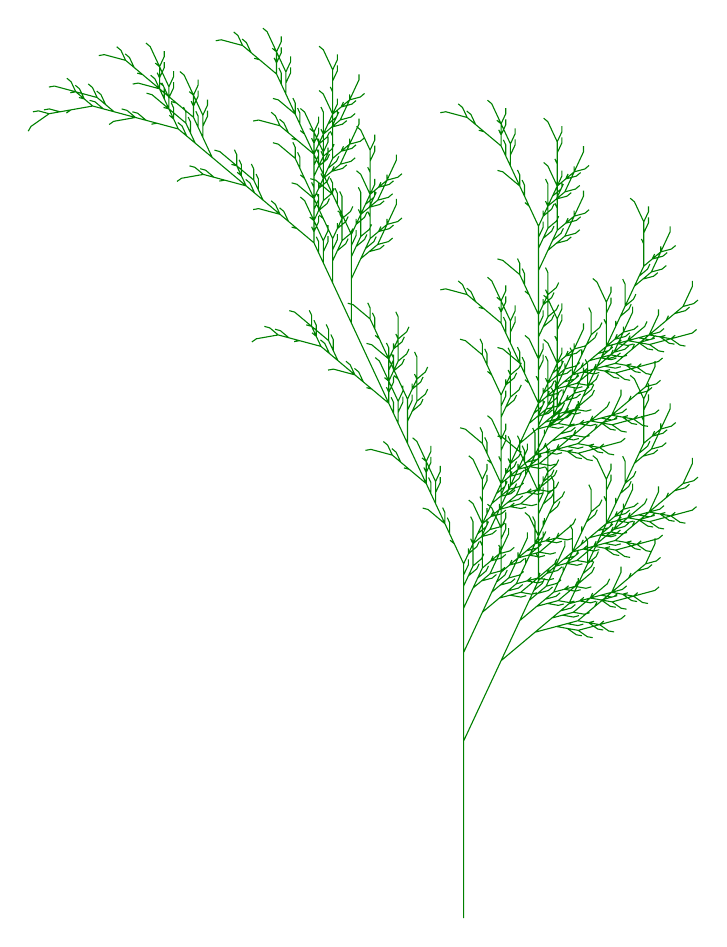
\begin{tikzpicture}
    \draw [green!50!black, rotate=90]
    [l-system={Fractal plant, axiom=X, order=6, step=2pt, angle=25}]
    lindenmayer system; 
\end{tikzpicture}
  \caption{\latex ile çizilmiş ağaç}
  \label{fig:ornekgrafik2}
\end{figure}

\section{\latex Yüklenmesi}
\latex yerel olarak bilgisayarlara kurulabileceği gibi, online platformlar üzerinden de kullanılmaktadır. Bilgisayar Mühendisliği olarak bizim tavsiyemiz \texttt{www.sharelatex.com} sitesinin kullanılmasıdır. Yapılması gereken proje koordinatörlüğü sayfasında verilen sıkıştırılmış \latex taslak dosyasının bu siteye yüklenmesidir. Online bu sistem, paket yükleme derdinden kurtardığı gibi doküman paylaşma özelliği ile birden fazla kişinin dokümanı inceleme ve düzenlemesine olanak sağlamaktadır. 

\chapter{Proje \latex Formatı}

Bu bölümde Yıldız Teknik Üniversitesi Bilgisayar Mühendisliği Bölümü'nün bilgisayar ve bitirme projeleri için kullanılacak \latex formatı tanıtılacaktır.

\section{Dosya Yapısı}
\latex formatı hazırlanırken, kullananların en az bilgi ile rahatça kullanabilecekleri bir şekilde olmasına dikkat edilmiştir. Bunun için anlaşılır bir dosya yapısı tercih edilmiştir. 

\begin{figure}[!ht]
  \centering
  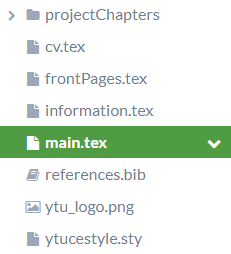
\includegraphics{zkilavuz/dosyayapisi}
  \caption{\latex taslağı dosya yapısı}
  \label{fig:dosyayapisi}
\end{figure}

Şekil-\ref{fig:dosyayapisi}, proje yazımı için tasarlanmış \latex taslağının dosya yapısını göstermektedir. Burada adı geçen dosya ve klasörleri şu şekilde inceleyebiliriz:

\begin{description}
    \item[main.tex] Tüm dosya yapısının başında yer almaktadır. Derleyici üzerinde bu kod çalıştırılmalıdır.
    \item[information.tex] Proje ile alakalı bilgilerin doldurulması gereken dosyadır. İlerleyen başlıklarda nasıl doldurulacağı anlatılacaktır.
    \item[references.bib] Proje içerisindeki referansların bulunduğu dosyadır. Referans işlemlerinin nasıl yapılacağı sonraki bölümlerde bahsedilecektir.
    \item[ytuthesis.sty] Proje için hazırlanmış sitil dosyasıdır. Bu dosya üzerinde değişiklik yapılmaması gerekmektedir.
    \item[frontPages.tex] dosyası, proje kitabının ön sayfalarında yer alan bölümleri içermektedir. Bu kısımdaki dosyaların değiştirilmemesi gerekmektedir \item[projectChapters] klasörü, proje kitabının içerisindeki bölümleri ve proje kitabında kullanılan resimleri içermektedir.
    \item[cv.tex] dosyası öğrenci özgeçmiş sayfasını oluşturmaktadır. Bu sayfa üzerinde değişiklik yapılmaması gerekmektedir.
\end{description}

\section{Proje Bilgilerinin Girilmesi}
Proje ile alakalı bilgiler \texttt{information.tex} dosyasında sorulduğu biçimi ile yazılacaktır. Tüm bilgi alanlarının formatı şu şekildedir:

\begin{minted}{latex}
% Asagidaki kisma .... yaziniz
\def\tanim{ Bu Kismi Doldurunuz }
\end{minted}

Yukarıda görüldüğü gibi, her bir bilgi üzerinde açıklama yer almaktadır. Bilgiler ise küme parantezleri ile gösterilen alanın arasına yazılmalıdır. Bu dosyada istenilen bilgileri şu şekilde sıralayabiliriz:

\begin{enumerate}
    \item \textbf{titleTR}, proje başlığı büyük harflerle Türkçe olarak yazılmalıdır.
    \item \textbf{titleEN}, proje başlığı büyük harflerle İngilizce olarak yazılmalıdır.
    \item \textbf{studenti}, projeyi yapan öğrencilerden ilkinin ismi ve soyismi yazılmalıdır. İsimlerin sadece ilk harfi büyük olmalıdır.
    \item \textbf{numberi}, projeyi yapan öğrencilerden ilkinin öğrenci numarası yazılmalıdır.
    \item \textbf{studentibdate}, projeyi yapan öğrencilerden ilkinin doğum tarihini ve doğum yeri yazılmalıdır.
    \item \textbf{studentiemail}, projeyi yapan öğrencilerden ilkinin e-posta adresi yazılmalıdır.
    \item \textbf{studentiphone}, projeyi yapan öğrencilerden ilkinin telefon numarası yazılmalıdır.
    \item \textbf{studentiintern}, projeyi yapan öğrencilerden ilkinin staj bilgileri yazılmalıdır.
    \item \textbf{studentii}, projeyi yapan öğrencilerden ikincisinin ismi ve soyismi yazılmalıdır. İsimlerin sadece ilk harfi büyük olmalıdır. Eğer ikinci öğrenci yoksa $\sim$ yazılmalıdır.
    \item \textbf{numberii}, projeyi yapan öğrencilerden varsa ikincisinin öğrenci numarası yazılmalıdır.
    \item \textbf{studentiibdate}, projeyi yapan öğrencilerden varsa ikincisinin doğum tarihini ve doğum yeri yazılmalıdır.
    \item \textbf{studentiiemail}, projeyi yapan öğrencilerden varsa ikincisinin e-posta adresi yazılmalıdır.
    \item \textbf{studentiiphone}, projeyi yapan öğrencilerden varsa ikincisinin telefon numarası yazılmalıdır.
    \item \textbf{studentiiintern}, projeyi yapan öğrencilerden varsa ikincisinin staj bilgileri yazılmalıdır.
    \item \textbf{date}, proje kitabının teslim edildiği tarih "ay, yıl" olarak yazılmalıdır. Burada ay, proje yazım dilinde kelime olarak yazılmalıdır.
    \item \textbf{advisorTR}, proje danışmanının ünvanı, ismi ve soyismi yazılmalıdır. Ünvan Türkçe olarak yazılmalıdır. İsimlerin ise sadece ilk harfleri büyük olmalıdır.
    \item \textbf{advisorEN}, proje danışmanının ünvanı, ismi ve soyismi yazılmalıdır. Ünvan İngilizce olarak yazılmalıdır. İsimlerin ise sadece ilk harfleri büyük olmalıdır.
    \item \textbf{acknowledgementText}, teşekkür metni proje yazım dilinde yazılmalıdır. 
    \item \textbf{abstractTextEnglish}, projenin özet bilgisi İngilizce olarak yazılmalıdır.
    \item \textbf{abstractKeywordsEnglish}, proje için geçerli olan anahtar kelimeler İngilizce olarak yazılmalıdır. Aralarına virgül konulmalıdır.
    \item \textbf{abstractTextTurkish}, projenin vözet bilgisi Türkçe olarak yazılmalıdır.
    \item \textbf{abstractKeywordsTurkish}, proje için geçerli olan anahtar kelimeler Türkçe olarak yazılmalıdır. Aralarına virgül konulmalıdır.
    \item \textbf{symbols}, tez içerisinde kullanılan semboller ve anlamları yazılmalıdır. "\mintinline{latex}{\item[sembol] Açıklaması}" şeklinde yazılmalıdır. Eğer tez içerisinde sembol kullanılmadıysa "\mintinline{latex}{\def\symbols{}}" olacak şekilde küme parantezleri içerisindeki metin silinmelidir.
    \item \textbf{abbrevations}, tez içerisinde kullanılan kısaltmalar ve anlamları yazılmalıdır. "\mintinline{latex}{\item[kısaltma] Açıklaması}" şeklinde yazılmalıdır. Eğer tez içerisinde kısaltma kullanılmadıysa "\mintinline{latex}{\def\abbrevations{}}" olacak şekilde küme parantezleri içerisindeki metin silinmelidir.
\end{enumerate}

Dikkat edilirse, isim içerisinde ayrım belirtilmediği sürece tüm bilgiler proje hangi dilde hazırlanıyorsa o dilde yazılmaktadır. 

\section{Proje Kitabı Ana Dosyasının Düzenlenmesi}\label{sc:Parametre}
Proje kitabı taslak hiyerarşisinin en üstündeki dosya \texttt{main.tex} dosyasıdır. Bu dosya üzerinde bazı düzenlemeler yapılması gerekebilmektedir.

Ana dosyanın içerisinde aşağıdaki gibi bir satır bulunmaktadır:

\begin{minted}{latex}
\usepackage[computer, final]{ytucestyle}
\end{minted}

Bu satırda köşeli parantezler içerisinde yer alan bilgiler yazılan proje ile alakalı bazı parametreleri göstermektedir. Verilebilecek iki farklı parametre vardır:

\begin{enumerate}
    \item \textbf{Projenin türü}: Hangi kademe için proje kitabı yazılıyorsa ona uygun olarak parametre verilmelidir. Bilgisayar projesi ise \textit{computer}, bitirme projesi ise \textit{senior} yazılmalıdır.
    
    \item \textbf{Projenin durumu}: Proje kitabı için bulunulan aşama belirtilmelidir. Eğer ara rapor verecekseniz \textit{report}, proje kitabının son halini teslim edecekseniz (final sınavı dahil) \textit{final} yazılmalıdır. Bu parametre üçüncü rapor teslimi için ya da başarılı not alan öğrencilerin teslim edeceği proje kitapları için kullanılmalıdır.
\end{enumerate}

Parametrelerin sırası önemsiz olmakla birlikte aşağıdaki örnekleri inceleyiniz:

\begin{itemize}
    \item \mint{latex}|\usepackage[computer, final]{ytuthesis}| 
    Bilgisayar projesinin final sınavı ve sonrası için teslim edilecek halini ifade etmektedir.
    \item \mint{latex}|\usepackage[senior, report]{ytuthesis}| 
    Bitirme projesinin ara raporları için teslim edilecek halini ifade etmektedir.
\end{itemize}

\section{Bölümler ve Ekler}
Tercihe bağlı olmakla birlikte, kullanıcıların dosyalarını daha rahat organize edebilmeleri için \texttt{projectChapters} isminde bir klasör oluşturulmuştur. Şekil-\ref{fig:bolumlerekler} bu klasörün içerisindeki dosyaları göstermektedir.

\begin{figure}[!ht]
  \centering
  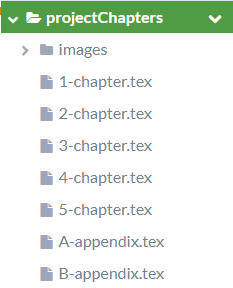
\includegraphics{zkilavuz/bolumlerekler}
  \caption{\texttt{projectChapters} klasör örneği}
  \label{fig:bolumlerekler}
\end{figure}

Şekil-\ref{fig:bolumlerekler}'ten görüldüğü üzere, proje için yazılması planlanan her bir bölüm veya ek ayrı bir \texttt{.tex} uzantılı dosya ile saklanmıştır. Tamamı tek bir \texttt{.tex} dosyasında da saklanabilir ancak bu durum yazma hakimiyeti azaltabilir. Aynı zamanda proje kitabı içinde kullanılacak resimler için \texttt{images} isimli bir klasör açılmıştır. 

\texttt{projectChapters} klasöründe bölümler/ekler için açılan her bir dosyanın \texttt{main.tex} içerisine eklenmesi gerekmektedir. 

\begin{figure}[!ht]
  \centering
  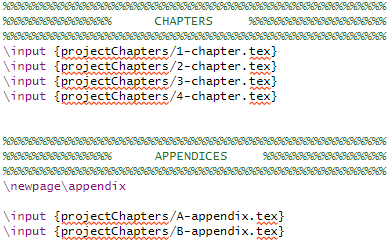
\includegraphics{zkilavuz/mainekleme}
  \caption{\texttt{main.tex} içine bölüm ve eklerin eklenmesi}
  \label{fig:mainekleme}
\end{figure}

Şekil-\ref{fig:mainekleme}'de görüldüğü gibi, eklenmek istenilen bölümler veya ekler \texttt{input} komutu ile \texttt{main.tex} içerisine eklenmektedir. Dosyalar hangi sıra ile verilirse, proje kitabının bölümleri o sırada oluşur.

\chapter{Semboller, Kısaltmalar ve Referanslar}

Bu bölümde sembollerin kısaltmaların ve referansların projenin \latex formatına nasıl ekleneceğinden bahsedilecektir:

\section{Semboller}
\texttt{information.tex} dosyasında yer alan \texttt{symbols} bilgisi içerisine şu formatta eklenmelidir: 

\begin{minted}{latex}
    \item[SEMBOL] Sembolun aciklamasi
\end{minted}

\texttt{item} komutundan sonra köşeli parantez içerisinde sembol, köşeli parantezden sonra, boşluk sayısı önemli olmaksızın, sembolün açıklaması yazılmalıdır. Verilen formata göre ilgili örnek aşağıda verilmiştir:

\begin{minted}{latex}
\begin{abbrv}
    \item[Ai]           Activities of Daily Life
    \item[c]            Alternate Step Test
    \item[C]            Body Mass Index
    \item[CR]           Cross Step moving on Four Stops
    \item[$fc(.)$]      Dynamic Bayesian Networks
    \item[$\Delta H$]   Demura's Fall Risk Assessment Chart
    \item[$\lambda i$]  Electromyography
\end{abbrv}
\end{minted}

Eğer proje raporu içerisinde sembol kullanılmıyorsa, "\mintinline{latex}{\def\symbols{}}" şeklinde küme parantezleri içerisi boş bırakılmalıdır.

\section{Kısaltmalar}
\texttt{information.tex} dosyasında yer alan \texttt{abbrevations} bilgisi içerisine şu formatta eklenmelidir: 

\begin{minted}{latex}
    \item[KISALTMA] Kisaltmanin aciklamasi
\end{minted}

\texttt{item} komutundan sonra köşeli parantez içerisinde kısaltma, köşeli parantezden sonra, boşluk sayısı önemli olmaksızın, kısaltmanın açıklaması yazılmalıdır. Verilen formata göre ilgili örnek aşağıda verilmiştir:

\begin{minted}{latex}
\begin{abbrv}
    \item[ADL]      Activities of Daily Life
    \item[AST]      Alternate Step Test
    \item[BMI]      Body Mass Index
    \item[CSFT]     Cross Step moving on Four Stops
    \item[DBN]      Dynamic Bayesian Networks
    \item[DFRAC]    Demura's Fall Risk Assessment Chart
    \item[EMG]      Electromyography 
\end{abbrv}
\end{minted}

Eğer proje raporu içerisinde kısaltma kullanılmıyorsa, "\mintinline{latex}{\def\abbrevations{}}" şeklinde küme parantezleri içerisi boş bırakılmalıdır.

\section{Referanslar}
Proje için tasarlanan \latex formatında referansların rahat eklenebilmesi ve kullanılabilmesi için \texttt{references.bib} dosyası oluşturulmuştur.

\subsection{Referans Dosyasının İsminin Değiştirilmesi}
\texttt{references.bib} dosyasının ismi değiştirilmek istenilirse, \texttt{main.tex} dosyasında yer alan şu satırda ilgili değişikliklerin yapılması gerekmektedir:

\begin{minted}{latex}
\addbibresource{references.bib}
\end{minted}

\subsection{\latex Formatında Referansların Oluşturulması}
Referansları elde etmenin en iyi yolu, referans gösterilecek kaynağın sitesinden \latex formatında referans bilgilerini almaktır. \texttt{scholar.google.com} adresi üzerinden de bu iş kolayca yapılmaktadır. İlgili kaynak site üzerinde aratıldığında çıkan her bir sonucun sağ alt köşesindeki "Alıntı Yap" seçeneğine tıklanmalıdır. Çıkan pencerenin sol alt köşesinde "BibTex" yazmaktadır. Buraya tıklanıldığında çıkan bilgilerin tamamı \texttt{references.bib} dosyasının içerisine  kaydedilmelidir. Örnek bir alıntı aşağıda gösterilmiştir:

\begin{minted}{latex}
@article{knauff2014efficiency,
  title={An Efficiency Comparison ...},
  author={Knauff, Markus and Nejasmic, Jelica},
  journal={PloS one},
  volume={9},
  number={12},
  pages={e115069},
  year={2014},
  publisher={Public Library of Science}
}
\end{minted}

Yukarıdaki örnek alıntı önemli olan ilk satırda yer alan \texttt{knauff2014efficiency} ifadesidir. Her alıntıda bu kısımda yer alan ifade anahtar kelimedir ve tüm alıntılar için burada yazılı olan ifadenin farklı olması gerekmektedir. (Buradaki ifadeleri siz de belirleyebilirsiniz). Bu anahtar kelimeler, metin içerisinde referans verilirken kullanılacaktır.

Bilgiler \texttt{references.bib} içerisine kaydedilirken sıra önemli değildir. Önemli olan projenin bölümleri içerisinde verilme sırasıdır. \latex numaralandırmayı bu düzene göre kendisi yapacaktır.

\subsection{Metin İçerisinde Referans Verme}
Metin içerisinde referans verirken, referans verilecek yere \texttt{cite} komutu ile alıntının anahtar kelimesi yazılır. Aşağıdaki örnek kullanımı inceleyiniz:

\begin{minted}[breaklines=true]{latex}
There are two airports in Istanbul. Ataturk Airport is on the European Side of the city, and Sabiha Gokcen Airport is on the Asian Side. As both of the airports are located outside the city centre you may find the taxi\cite{rao2012novel} fees fairly expensive. 
\end{minted}

Eğer birden fazla kaynak gösterilecekse; anahtar kelimeler virgül ile ayrılarak tek bir adet \texttt{cite} içerisine yazılmalıdır. Aşağıdaki örneği inceleyiniz:

\begin{minted}[breaklines=true]{latex}
There are two airports in Istanbul. Ataturk Airport is on the European Side of the city, and Sabiha Gokcen Airport is on the Asian Side. As both of the airports are located outside the city centre you may find the taxi\cite{rao2012novel, knauff2014efficiency, brischoux2009don} fees fairly expensive. 
\end{minted}

\chapter{Tablolar, Şekiller ve Matematiksel İfadeler}

Bu bölümde \latex için tablo ve resim eklemekten bahsedilecektir.

\section{Tablolar}
\latexx'e tablo eklemek için temel olarak aşağıdaki komut kullanılmaktadır:

\begin{minted}{latex}

\begin{table}[yerlesim]
    \centering
    \caption{My caption}
    \label{mylabel}
    
    TABLO

\end{table}

\end{minted}

Yukarıdaki kodlardan görüleceği üzere, bir tablo eklemek için dört bilgiye ihtiyaç vardır: 

\begin{enumerate}
    \item Yerleşim: Tablonun sayfanın neresine yerleşeceği bilgisi verilir. Bu bilginin nasıl olacağı daha sonra açıklanacaktır.
    \item \texttt{caption}: Tablonun açıklaması kısmında yazılacak bilgiler
    \item \texttt{label}: Tabloya referans verilmesi için gerekli olacak anahtar kelime
    \item Tablo: Tablonun kendisi. Burada herhangi bir bilgi tablo olarak eklenebilmektedir. Ancak satır, sütun mantığı ile en temel tablo \texttt{tabular} komutu ile eklenmektedir.
\end{enumerate}

\texttt{www.tablesgenerator.com} web sayfası \latexx'e yeni başlayan kullanıcılar için tablo oluşturma konusuda yardımcı olmaktadır. Bu site üzerinden tablonun kodları oluşturulup proje kitabına eklenebilir. Bu site kodları oluştururken yerleşim kısmını boş bırakmaktadır. Bu kısmı sizin doldurmanız gerekmektedir.

\section{Şekiller}
\latexx'e şekil eklemek için temel olarak aşağıdaki komut kullanılmaktadır:

\begin{minted}{latex}

\begin{figure}[yerlesim]
    \centering
    
    SEKIL

    \caption{My caption}
    \label{mylabel}
\end{figure}

\end{minted}

Yukarıdaki kodlardan görüleceği üzere, bir şekil eklemek için dört bilgiye ihtiyaç vardır: 

\begin{enumerate}
    \item Yerleşim: Şeklin sayfanın neresine yerleşeceği bilgisi verilir. Bu bilginin nasıl olacağı daha sonra açıklanacaktır.
    \item Şekil: Şeklin kendisi. Burada herhangi bir bilgi şekil olarak eklenebilmektedir.
    \item \texttt{caption}: Şeklin açıklaması kısmında yazılacak bilgiler
    \item \texttt{label}: Şeklin referans verilmesi için gerekli olacak anahtar kelime
\end{enumerate}

Burada tablolardan farklı olarak \texttt{caption} bilgisi aşağıda yer almıştır. \texttt{caption} bilgisi nerede yer alırsa, şeklin ya da tablonun açıklaması ona göre yer değiştirmektedir.

Şekil kısmına resim ekleme şu şekilde yapılabilir:

\begin{minted}{latex}
    \includegraphics[scale=0.6]{projectChapters/images/Picture1.png}
\end{minted}

Bu komut ile \texttt{projectChapters} klasörü içerisinde oluşturulan \texttt{images} klasöründeki \texttt{Picture1.png} dosyası eklenmiştir. Eklenirken \texttt{scale} komutu ile boyutu \%60'a indirgenmiştir. Eğer resmi metin uzunluğuna göre boyutlandırmak istiyorsanız komut aşağıdaki gibi yazılmalıdır:

\begin{minted}{latex}
    \includegraphics[width=0.2\textwidth]{projectChapters/images/Picture1.png}
\end{minted}

Bu komut ile resmin ekleneceği yerdeki metin uzunluğunun \%20'si kadar olacak şekilde resmin genişliğini ayarlar. Resmin genişliği ile aynı oranda enide ayarlanmış olur. 

\section{Tablo ve Şekillerin Sayfa Yerleşimi}
Bu bilgi tablo ve şekillerin dokümanın neresine yerleştirilmesi gerektiğini bildirmektedir:

\begin{itemize}
    \item \textbf{h}: Yaklaşık olarak buraya yerleştir (here)
    \item \textbf{t}: Sayfanın en üstüne yerleştir (top)
    \item \textbf{b}: Sayfanın en altına yerleştir (bottom)
    \item \textbf{p}: Özel bir sayfaya yerleştir
    \item \textbf{!}: Genelleştirilmiş parametreleri burada yoksay.
    \item \textbf{H}: Kesin olarak buraya yerleştir. \texttt{h!} komutuna karşılık gelmektedir.
\end{itemize}

Bu bilgilerin biri veya birkaçı verilerek yerleşim sağlanmaktadır. Birden fazla olduğu durumda sırası ile uygun olan yerleşimi yapmaktadır. Aşağıdaki örneği inceleyiniz:

\begin{minted}{latex}

\begin{figure}[!htbp]
  \centering
  \includegraphics{projectChapters/images/Picture1.png}
  \caption{Ornek resim ekleme}
  \label{anahtarkelime}
\end{figure}

\end{minted}

\section{Anahtar Kelimeler ve Referans Verme}\label{sc:refref}
Eklenen tablo veya şekle metin içerisinden referans verebilmek için ekleme sırasında \texttt{label} komutu ile anahtar kelime ataması yapılmıştı.

Anahtar kelimeler boşluksuz ve İngiliz alfabesinin karakterlerinden oluşan kelimeler olmalıdır. Birçok latex kullanıcısı, anahtar kelimenin neye ait olduğunu rahat anlamak için anahtar kelimelerin önüne bazı tanımlayıcılar koyarlar (Not: Bu işlem zorunlu değildir). Örneğin tablonun anahtar kelimesi ise \texttt{tab:}, şeklin anahtar kelimesi ise \texttt{fig:} tanımlayıcısını kullanırlar. Böylece metin içerisinde referans verilen bilginin tablo mu, şekil mi olduğu anlaşılmaktadır.

Metin içerisinde referans verirken \texttt{ref} komutu kullanılmaktadır. Bu komutun içerisine anahtar kelime yazılmalıdır. \texttt{ref} komutu ile tablo veya şeklin sadece numarası alındığından bu komut öncesinde \textit{tablo} veya \textit{şekil} kelimeleri yazılmalıdır. Aşağıdaki örneği inceleyiniz:

\begin{minted}{latex}
Haydi bir resim ekleyelim:

\begin{figure}[!ht]
  \centering
  \includegraphics{projectChapters/images/Picture1.png}
  \caption{Resim ekleme ornegi}
  \label{fig:ornekresim}
\end{figure}

Resim-\ref{fig:ornekresim}, ornek bir haritadir.
\end{minted}

\section{Matematik Formülleri}
\texttt{www.codecogs.com/latex/eqneditor.php} web sayfası üzerinden matematik formüllerinizi kolayca oluşturup, elde edilen kodları buraya ekleyebilirsiniz. Elde edilen kodlar numaralandırılarak eklenecekse şu şekilde eklenmelidir:

\begin{minted}{latex}
\begin{equation}
    Denklem Kodlari
\end{equation}
\end{minted}

Eğer metin içerisinde matematiksel ifade kullanılacaksa \$ işaretleri arasına yazılmalıdır. Örneğin $\frac{3}{2}$ yazmak için \mint{latex}|$\frac{3}{2}$| yazılmalıdır.

\chapter{Listeleme ve Maddeleme}
Bu bölümde \latex kullanarak listeleme ve maddeleme işlemleri gösterilecektir.

\section{Listeleme}
Listeleme yapmak için aşağıdaki komut yazılır:

\begin{minted}{latex}
\begin{itemize}
    \item Birinci madde
    \item İkinci madde
    \item Üçüncü madde
\end{itemize}
\end{minted}

Yukarıdaki komut çalıştırıldığında aşağıdaki sonuç çıkacaktır:

\begin{itemize}
    \item Birinci madde
    \item İkinci madde
    \item Üçüncü madde
\end{itemize}

\section{Maddeleme}
Numaralandırma yaparak maddeleme yapabilmek için aşağıdaki komut yazılır:

\begin{minted}{latex}
\begin{enumerate}
    \item Birinci madde
    \item İkinci madde
    \item Üçüncü madde
\end{enumerate}
\end{minted}

Yukarıdaki komut çalıştırıldığında aşağıdaki sonuç çıkacaktır:

\begin{enumerate}
    \item Birinci madde
    \item İkinci madde
    \item Üçüncü madde
\end{enumerate}

\section{İç içe maddelemeler}
İç içe listeler veya numaralandırılmış listeler oluşturulmak istenildiğinde belirtilen komutlar iç içe yazılması yeterli olacaktır. Örneğin;

\begin{minted}{latex}
\begin{itemize}
    \item Birinci seviye, maddeleme, birinci madde
    \begin{itemize}
        \item İkinci seviye, maddeleme, birinci madde
        \item İkinci seviye, maddeleme, ikinci madde
        \begin{enumerate}
            \item Üçüncü seviye, numaralandırma, birinci madde
            \item Üçüncü seviye, numaralandırma, ikinci madde
        \end{enumerate}
    \end{itemize}
    \item Birinci seviye, maddeleme, ikinci madde
\end{itemize}
\end{minted}

Yukarıdaki komut çalıştırıldığında sonuç aşağıdaki gibi olacaktır:

\begin{itemize}
    \item Birinci seviye, maddeleme, birinci madde
    \begin{itemize}
        \item İkinci seviye, maddeleme, birinci madde
        \item İkinci seviye, maddeleme, ikinci madde
        \begin{enumerate}
            \item Üçüncü seviye, numaralandırma, birinci madde
            \item Üçüncü seviye, numaralandırma, ikinci madde
        \end{enumerate}
    \end{itemize}
    \item Birinci seviye, maddeleme, ikinci madde
\end{itemize}

\chapter{Proje Kitabı Nasıl Yazılır?}

Bu bölümde proje kitaplarının nasıl yazılacağı hakkında bilgi verilecektir.

\section{Genel Yazım Kuralları}

Proje kitabı ve ara raporlar rahat anlaşılır, dil bilgisi ve yazım kurallarına uygun ve basit bir dille yazılmalıdır. Cümlelerin mümkün olduğunca kısa ve fiil zamanlarının uyumlu olması anlatımı kolaylaştıracaktır. Yazılanlarda anlam ve anlatım bütünlüğüne dikkat edilmelidir. Özellikle İngilizce yazılan raporlarda kaynaklardan kopyala- yapıştır metoduyla bilgi kesinlikle alınmamalıdır. Alınacak bilgi yorumlanarak yeniden yazılmalı ve kaynağa atıfta bulunulmalıdır.

Proje kitabı tamamlanmış bir çalışmayı anlattığı için öğrenilen (miş’li) geçmiş zaman kullanılmalıdır. Proje çalışması edilgen bir yapıda (yapılmıştır, kullanılmıştır gibi) anlatılmalıdır. Genel bilgiler ise geniş zaman kullanılarak (yapılır, eklenir gibi) verilmelidir.

\section{Proje Kitabının Bölümleri}

Genellikle proje kitabını okuyanlar, her ana bölümün ilk paragrafını okuyarak o bölüm hakkında fikir sahibi olmaya çalışırlar. Bunun için Giriş bölümünden sonra her ana bölümün ilk paragrafı o bölümü ana hatlarıyla tanıtmalıdır.

Aşağıda verilecek bölümlerin içerikleri projenin kapsamı ve gerçekleştirilen sistemin yapısına bağlı olarak değişiklikler gösterebilir. Ancak her proje için bu başlıklar yer almalıdır. Örneğin bir web uygulaması için uygulama bölümünde çok sayıda ekran çıktısına yer verilirken, performans analizi başlığında verilen bilgi sayfaların açılma süreleri veya uygulamanın tepki süresinin ölçülmesiyle sınırlı kalabilir. Öte yandan akademik sonuçlar üretmeye yönelik bilimsel yöntemler içeren bir çalışmada bunun tam tersi bir yapı söz konusu olacak ve deneysel sonuçlar ile performans analizleri yoğun içeriğe sahip olacaktır. 

Proje Kitabı şablonuna uygun olarak proje kitabı içerisinde bulunması gereken bölümler ve sıralaması aşağıda verilmiştir:

\subsection{Kapak Sayfası}
Bu kısım \latex tarafından oluşturulmaktadır.
\subsection{Telif Hakkı Devir Sayfası}
Bu kısım \latex tarafından oluşturulmaktadır.
\subsection{Teşekkür} 
Bu kısım, uzun bir çalışmayı tamamlayan ekibin, projenin teknik ve bilimsel içeriğinden bağımsız olarak görüşlerini yazdığı bölümdür. Ayrıca bu bölümde, proje çalışması sırasında bilgi, kaynak v.b. yardımı alınan kişi ve kuruluşlara teşekkür edilmelidir. Bu bölümde, çalışmasını tamamlayan ekip kendisine/kendilerine destek olan, yardım eden ailelerine ve arkadaşlarına da ayrıca teşekkür edebilir.

\texttt{information.tex} dosyası içerisinde ilgili kısım doldurulduğunda \latex tarafından oluşturulmaktadır.

\subsection{İçindekiler}
Bu kısım \latex tarafından oluşturulmaktadır.
\subsection{Simge Listesi}
\texttt{information.tex} dosyası içerisinde ilgili kısım doldurulduğunda \latex tarafından oluşturulmaktadır. Eğer sembol kullanılmıyorsa \texttt{information.tex} dosyasındaki ilgili kısım boş bırakılmalıdır.

\subsection{Kısaltma Listesi}
\texttt{information.tex} dosyası içerisinde ilgili kısım doldurulduğunda \latex tarafından oluşturulmaktadır. Eğer kısaltma kullanılmıyorsa \texttt{information.tex} dosyasındaki ilgili kısım boş bırakılmalıdır.

\subsection{Şekil Listesi}
Bu kısım \latex tarafından oluşturulmaktadır.
\subsection{Tablo Listesi}
Bu kısım \latex tarafından oluşturulmaktadır.
\subsection{Özet} 
Bir proje kitabının en çok okunan bölümleri özet, giriş ve sonuç bölümleridir. Konu hakkında sadece genel bilgi edinmek isteyen kişiler çoğunlukla bu üç bölümü okumakla yetinirler. Bunun için proje konusu ve elde edilen önemli sonuçlar özet, giriş ve sonuç bölümlerinde bölüm özelliğine uygun detayda yinelenmelidir.
    
Özetin amacı, okuyucunun proje konusu hakkında genel bir fikir sahibi olmasını sağlamaktır. Özetin ilk paragrafında proje konusu tanıtılmalıdır. Diğer paragraflarda çalışmanın motivasyonu (çalışmanın neden yapıldığı), kapsamı, amacı ve katkısı adım adım anlatılmalı, kullanılan yöntemler kısaca tanıtılmalı ve ana sonuçlar verilmelidir.

Özet, tamamlanmış bir çalışmayı anlattığı için öğrenilen (miş’li) geçmiş zaman kullanılmalıdır. Anlatım, “yapılmıştır, tamamlanmıştır” gibi edilgen yapıda olmalıdır.

\texttt{information.tex} dosyası içerisinde ilgili kısım doldurulduğunda \latex tarafından oluşturulmaktadır.

\subsection{Abstract}

Bu bölüm, Özet bölümünün birebir İngilizce çevirisi olmalıdır. Bölümümüze değişim programlarıyla ve yabancı öğrenci kontenjanlarıyla gelen öğrenciler ancak Abstract bölümünü okuyarak Bilgisayar Projeleri hakkında bilgi sahibi olabilmektedirler. Bu sebeple çevirinin özenli yapılması, hazır çeviri araçlarıyla yetinilmemesi projenin hitap edeceği kitleyi uluslararası ölçeğe taşıyacaktır.

\texttt{information.tex} dosyası içerisinde ilgili kısım doldurulduğunda \latex tarafından oluşturulmaktadır.
    
\subsection{Giriş} 
Giriş bölümü, okuyucunun konuyu anlayıp projenin amacını ve konuya nasıl bir katkıda bulunduğunu değerlendirebilmesi için yeterli temel bilgileri içermelidir. Bu amaçla projenin konusu tanımlanmalı, çalışmanın yapılmasının gereği, amacı ve hedefi kısaca anlatılmalıdır.
    
Projenin motivasyonu; bir başka deyişle, bu konunun seçiliş sebebi ve konunun neden önemli olduğu, giriş bölümünde iyi bir şekilde vurgulanmalıdır. Ayrıca projenin konuya olan özgün katkısı varsa giriş bölümünde açık bir şekilde anlatılmalıdır. Bunların yanında proje çalışmasının anlaşılabilmesi için bilinmesi gereken ön bilgiler, giriş bölümünde okuyucuya aktarılmalıdır.

Giriş bölümünün sonunda okuyucunun hangi bölümleri okuyacağına karar vermesini kolaylaştırmak için proje kitabının sonraki bölümleri kısaca tanıtılmalıdır.

\subsection{Ön İnceleme} 
Ön inceleme bölümü, projenin yapılacağı alanda daha önceden yapılmış olan mevcut ve benzeri çalışmaların incelenmesini içerir. Ön incelemenin amacı, projenin önceki çalışmalardaki hangi eksikleri gidereceği ya da hangi yolun izleneceğinin belirlenmesidir. Proje alanının etüt edilmesi ile kabaca gerçekleştirilecek projenin hangi ihtiyaçlara cevap vereceği belirlenir.
    
Bu bölümde konu ile ilgili daha önce yapılmış olan çalışmalar anlatılmalı ve değerlendirmeleri yapılmalıdır. Bilimsel ve akademik içerikli çalışmalarda literatür özeti olarak bilinen bu bölümde konunun daha önceden hangi yönleriyle ele alınarak hangi sonuçların elde edildiği karşılaştırmalı olarak değerlendirilir. Bu sayede konuda uygulanan yöntemler ve eksik yönler ortaya çıkarılmış olur.

Bilgi sistemi ya da web uygulaması gibi projelerde halihazırda işlerin nasıl yürüdüğü anlatılmalı, aynı konuda yapılmış benzer sistemler ve örnekler karşılaştırmalı olarak değerlendirilmelidir. Bunların çalışma ilkeleri ve özellikleri, varsa eksik yönleri ve projenin bu alanda ne katkı sağlayacağı belirtilmelidir.

\subsection{Fizibilite} 
Fizibilite bölümünde projenin yapılabilirlik etüdü gerçekleştirilmelidir. Projenin başarıya ulaşması için kaynakların alternatifler arasından hangi şartlara uygun olarak nasıl seçildiği, projenin zaman planlaması, projenin ekonomik öngörüleri ve yapılması durumunda oluşacak katma değerler bu bölümde incelenir ve belirlenir. Genel olarak Fizibilite çalışması,
    
    \begin{itemize}
        \item \textbf{Teknik Fizibilite:} Teknik fizibilite, marka bağımsız teknik özelliklerin vurgulandığı bir çalışma olup kendi içinde Yazılım Fizibilitesi, Donanım Fizibilitesi ve Haberleşme (İletişim) Fizibilitesi şeklinde gruplanabilir.
        
Yazılım Fizibilitesi başlığında, kurulacak sistemi oluşturmak üzere seçilen İşletim Sistemi, Veri Tabanı Yönetim Sistemi, Web Sunucusu ve/veya diğer sunucu sistemleri, Uygulama Geliştirme Dili, Uygulama Geliştirme Ortamı, Diğer Ek Destek Yazılım Araçları gibi yazılım unsurlarının neler olduğunun ve bu unsurlarda ne tür teknik özellikler beklendiğinin vurgulanması gereklidir. Bu yazılım unsurlarının doğal olarak marka bağımlı alternatifleri de vardır. Beklenen teknik özelliklere göre hangi alternatifin seçildiği karşılaştırmalar yaparak ortaya konmalıdır. Bu durumda seçilen alternatifin neden diğerlerinden üstün olduğu somut nedenlere dayanarak vurgulamalıdır.

Donanım Fizibilitesinde hedef, yazılım fizibilitesinde seçilen yazılım unsurlarını ve bu unsurlar kullanılarak gerçekleştirilecek olan uygulamayı başarı ile çalıştırmaya müsait, kısa ve orta vadeli gelişmelere açık bir sistemin seçilmesidir. Kullanılacak yazılım araçları için en düşük sistem gereksinimleri (İşlemci hızı, RAM ihtiyacı, Disk ihtiyacı vb.) göz önüne alınarak bir kurulum belirlenmelidir. Ancak gerek teknolojinin geldiği nokta gerek ise işleyişin rahat olması için bu belirlenen özelliklerden daha iyi bir kurulum önerilmelidir. Bu fizibilite tamamen teknik veriler ışığında yapılabilir ve marka belirtilmesi gerekmez. Uygulamanın özel bir donanıma bağlı olarak yapılmasının gerekli olduğu durumlarda Yazılım Fizibilitesi donanımın özellikleri göz önüne alınarak hazırlanabilir.

İletişim Fizibilitesi başlığı altında iletişim teknolojileri ve buna bağlı olarak kullanılması uygun olan cihaz/yazılım vb. teknik özellikler incelenmelidir.
        \item \textbf{İş gücü ve Zaman Planlaması:} İş gücü ve Zaman planlaması yapılırken sonuca ulaşmak için takip edilecek ara adımlar tam olarak belirlenmeli ve bu adımların hangi teknik bilgi birikimine sahip kişilerce ve ne kadar sürede yapılabileceği yönünde planlar oluşturulmalıdır. Bu plan Gantt diyagramı kullanılarak ifade edilmelidir.
        
        \item \textbf{Yasal Fizibilite:} Yasal Fizibilite, yapılan işin mevcut kanun ve yönetmeliklere uygun olup olmadığı, herhangi bir patent vb. korunmuş hakkı ihlal edip etmediği ve/veya bazı teknolojililerin kullanılması için alınması gereken izinlerin olup olmadığı gibi unsurları değerlendirmek için yapılmalıdır. Eğer bu unsurlar söz konusu değilse Yasal Fizibilite yapılamaz.
        
        \item \textbf{Ekonomik Fizibilite:} Ekonomik Fizibilitede, teknik (yazılım, donanım, iletişim), iş gücü/zaman fizibilitesi ve yasal fizibiliteden doğacak harcamalar detaylandırılmalı ve projenin toplam giderleri ortaya konmalıdır. Bunun yanında projenin devreye alınması ile sağlanacak tasarruf ya da elde edilecek gelirler de öngörülerek mali gelir analizi yapılmalıdır. Gelir ve gider kalemleri başabaş noktası grafiği gibi yöntemlerle karşılaştırılarak sistemin harcamaları ne kadar sürede amorti edeceği gösterilebilir.
        
    \end{itemize}

başlıklarını içermelidir. Bunlar dışında olabilecek sosyal, alternatif vb. fizibilite çalışmaları proje ihtiyaçlarına bağlı olarak proje danışmanı yönlendirmesiyle eklenmelidir.

\subsection{Sistem Analizi} 
Sistem analizinin amacı projede en uygun çözümü bulmak için ana öğeler ve işlevlerin ortaya çıkarılıp tanımlanmasıdır. Bu bölümde projenin hedefleri detaylandırılır. Ayrıca bilgi kaynakları ve gereksinimler belirlenir. Bölüm sonunda proje ile ilgili tüm gereksinimler tanımlanmış ve tasarım aşamasına geçecek en uygun çözüm belirlenmiş olmalıdır.
    
Gereksinimlerin ortaya çıkarılması için kullanılan araştırma ve bilgi toplama yöntemleri (görüşme, anket, vb.) ve sonuçları bu bölümde verilmelidir. Belirlenen gereksinimler ışığında sistemdeki modüller, kullanıcılar ve roller tanımlanmalıdır.

Gereksinim analizi modeli fonksiyonel ya da nesneye dayalı olarak hazırlanabilir. Eğer fonksiyonel yaklaşım tercih edilirse, sistemin nasıl çalışacağına dair iş akışları ve analiz modeline ait veri akış diyagramları hazırlanmalıdır. Veri akış diyagramları ikinci düzeye kadar hazırlanmalı ve modüllerin analizi yapılmalıdır. Nesneye dayalı analiz tercih edildiğinde ise kullanım senaryoları (use-case) çözümlemesi ile gereksinimler belirlenmeli, kavramsal sınıf diyagramı ile analiz modeli oluşturulmalıdır.

Sistem analizi sonucunda proje sonlandığında ihtiyaçların karşılanıp karşılanmadığını test edecek yapı da ortaya çıkmaktadır. Bu sebeple projede kullanılacak performans metrikleri (hız, tanıma başarısı, özellik sayısı, vb.) de bu bölümde tanımlanmalıdır.

\subsection{Sistem Tasarımı} 
Analiz aşaması bittikten sonra gerçekleştirilen tasarım aşaması bu bölümde raporlanmalıdır. Bu bölüm temel olarak; yazılım tasarımı, veritabanı tasarımı ve girdi-çıktı tasarımı alt bölümlerinden oluşmalıdır.

\subsubsection{Yazılım Tasarımı}
Yazılım tasarımında, projede gerçekleştirilecek sistemin mimari tasarımı oluşturulmalıdır. Proje, bilgi sistemi gibi bir yazılım projesi ise bu bölüm sistem tasarımı ilkelerine göre hazırlanmalıdır. Proje, bilimsel bir sonuç veya deney için hazırlanıyorsa o zaman uygulanan bilimsel yöntem ve metodolojiler sırası ile tanıtılarak sistem tasarlanmalıdır.

Yazılım projelerinin tasarımı, bir önceki bölümde olduğu gibi bu alt bölüm de fonksiyonel ya da nesneye dayalı yaklaşımlarla hazırlanabilir. Fonksiyonel yaklaşım tercih edilecek ise veri akış diyagramlarından hareketle modüller hazırlanır ve yapı diyagramları ile tasarlanır. Nesneye dayalı tasarım, etkileşim diyagramları ile (ardışıl diyagramlar veya işbirliği diyagramları) yapılmalıdır. Bu aşamada yazılım sınıfları da ortaya çıkarılarak tasarım sınıf diyagramı da hazırlanmalıdır.

Bilimsel ve akademik çalışmalardan oluşan projelerde ise öncelikle, sistemin genel yapısı ve çalışma şekline ait blok diyagramı verilmelidir. Daha sonra, verilere uygulanan ön işleme adımları, kullanıldıysa özellikler üzerinde yapılan hazırlık işlemleri (özellik çıkarımı gibi), uygulanan yöntemler (sınıflandırma, kümeleme, zaman serisi tahmini, vb.) gibi bileşenler ayrıntılarıyla anlatılmalı ve blok diagramındaki her ana işlem aşamasında yapılan çalışmalara ait teknik bilgi ve gerekli yarı kod ve/veya akış diyagramı verilmeli, parametre seçimi, algoritma özelleştirme adımları gibi konular detaylı olarak anlatılmalıdır.

\subsubsection{Veritabanı Tasarımı}
Veritabanı tasarımında, projenin analiz ve tasarım aşamalarında belirlenen, hakkında veri tutulması gereken varlıklar ve bunlar arasındaki ilişkiler ortaya koymak için varlık-ilişki diyagramı (Entity-Relationship, E-R) kullanılmalıdır. Varlıklar ve aralarındaki ilişkiler tasarlandıktan sonra, eğer gerekiyorsa veri üzerinde veritabanı düzeyinde işlem yapmak için gerekli olan yordamlar (stored procedures) da tasarlanmalıdır. Veri üzerinde olay ve durumlara göre otomatik tetiklenerek çalışması gereken işlemler (trigger) de oluşturmalıdır.

Bilimsel veya akademik içerikli projelerde ise kullanılan veri kümeleri, özellikleri ve yapılarıyla tanıtılmalıdır. Veri kümeleri oldukları haliyle kullanılmayıp üzerinde seçme ya da azaltma gibi işlemler yapıldıysa bu bölümde açıklanmalıdır. Veri yapıları ve saklama biçimleri bu bölümde tariflenmelidir.

\subsubsection{Girdi-Çıktı Tasarımı}
Bu bölümde projenin veri girişlerini, işlem kontrollerini ve sonuç çıktılarını sağlayan ekranlar gibi arayüzlerin tasarımları verilmelidir. Uygulama penceresi, web sayfası, mobil cihaz arayüzü gibi çeşitli girdi ortamlarından hangileri kullanıldıysa bu bölümde yer almalıdır. Çıktı için form, rapor veya grafik gibi değişik ortamlar kullanılıyorsa bunların tasarımları da bu bölümde verilmelidir.

\subsection{Uygulama}
Bu bölümde gerçeklenen projenin çalışan haline ait ekran görüntüleri yer almalıdır. Özellikle gereksinimleri karşılayacak şekilde modül veya işlemlerin gösterilmesi beklenmektedir. Uygulamada yapılan kontroller, gerekirse her adımdan sonra ara çıktılar, girilen verinin sonucunda sistemin işlemesi ve elde edilen çıktılar gibi sistemin çalışan hali bu bölümde verilmelidir.


\subsection{Deneysel Sonuçlar}
Yazılım uygulamalarında sistemin değişik senaryolarla çalışması sonucunda oluşan çıktılar bu bölümde verilmelidir. Genel senaryoların dışında problemin uç noktaları gözönünde bulundurularak sistemin her koşul için girdi-çıktı uyumuna sahip olup olmadığı incelenmelidir.
Gerçekleştirilen uygulamada, farklı parametreler kullanılarak yapılan testlere ait sonuçların, farklı yöntemlerle elde edilen sonuçların, ya da farklı veri kümeleri üzerindeki uygulamaların karşılaştırmalı sonuçlarının bu bölümde verilmesi gereklidir.


\subsection{Performans Analizi}
Sistemin çalışma performansı bu bölümde değerlendirilmelidir. Performans değerlendirme için kullanılan yöntemler tanıtılmalı (örneğin stres testi) ve sonuçları tartışılarak değerlendirilmelidir.

Bilimsel içerikli projelerde ise bir önceki bölümde elde edilen deneysel sonuçlar değerlendirilmeli ve karşılaştırmalı olarak yorumlanmalıdır. Hangi yöntem veya parametre seti ile nasıl başarı sağlandığı, başarının neden yüksek ya da düşük olduğu objektif olarak yorumlanmalıdır.

\subsection{Sonuç}

Sonuç bölümü, gerçekleştirilen çalışmadan elde edilen sonuçların değerlendirildiği bölümdür. Bu bölümde;
\begin{itemize}
    \item Proje konusu tanımlanmalı ve kullanılan yöntemler özetlenmelidir.
    \item Elde edilen sonuçlar açık ve basit cümlelerle ifade edilmelidir.
    \item Deneysel çalışmalarda, farklı deney sonuçlarının değerlendirilmesinden elde edilen ana sonuçlar
    anlatılmalı mümkünse bu sonuçlara göre genellemeler yapılmalıdır.
    \item Bu konuda çalışmak isteyenlere yol göstermek için yapılan proje çalışmasında başlangıçta belirlenen
    hedefe ne kadar ulaşıldığı, çalışmanın üstün ve eksik yönleri anlatılmalıdır.
    \item İleriye yönelik çalışmalar için, varsa öneriler belirtilmelidir.
\end{itemize}

\subsection{Ekler}
Proje kitabınızda ihtiyaç duyulursa ekler bölümünde, proje metni içinde yer alması gerekli olmayan ve okunurluğu bozacak kadar büyük ve detaylı tablo, akış diyagramı gibi bilgiler bulunmalıdır. Bu bilgilere proje metni içinde gerektiği yerde referans verilmelidir.

\subsection{Referanslar}
Bu kısım \latex tarafından oluşturulmaktadır.

\subsection{Özgeçmiş}
\texttt{information.tex} dosyası içerisinde ilgili kısım doldurulduğunda \latex tarafından oluşturulmaktadır.

\chapter{Proje Raporlarının İçerikleri}

Dönem içerisinde iki adet rapor teslim edilmektedir. Bu iki rapordan sonra geçer not alan öğrenciler proje kitabını teslim etmektedirler. Raporlar projenin gelişme durumunu ifade etmektediler. Raporlarda yer alması gereken başlıklar şu şekildedir:

\subsubsection*{Ara Rapor}

Ara Raporda yer alması gereken bölümler aşağıdaki gibidir:
\begin{itemize}
\item İçindekiler Listesi  \hfill \textit{(taslak tarafından otomatik oluşturulmaktadır)}
\item Simge Listesi \hfill \textit{(\texttt{information.tex} dosyasını doldurmalısınız)}
\item Kısaltma Listesi \hfill \textit{(\texttt{information.tex} dosyasını doldurmalısınız)}
\item Tablo Listesi \hfill \textit{(taslak tarafından otomatik oluşturulmaktadır)}
\item Şekil Listesi \hfill \textit{(taslak tarafından otomatik oluşturulmaktadır)}
\item Giriş
\item Ön İnceleme 
\item Fizibilite
\item Sistem Analizi 
\item Sistem Tasarımı
\item Uygulama
\item Referanslar \hfill \textit{(taslak tarafından otomatik oluşturulmaktadır)}
\end{itemize}

\subsubsection*{Final Raporu}

Final Raporu, Ara Raporda yer alan bölümlere ek olarak şu bölümleri içermelidir:

\begin{itemize} 
\item Teşekkür \hfill \textit{(\texttt{information.tex} dosyasını doldurmalısınız)}
\item Özet \hfill \textit{(\texttt{information.tex} dosyasını doldurmalısınız)}
\item Abstract \hfill \textit{(\texttt{information.tex} dosyasını doldurmalısınız)}
\item Deneysel Sonuçlar
\item Performans Analizi 
\item Sonuç
\end{itemize}

Bölüm-\ref{sc:Parametre}'de belirtilen kurallara göre \latex kendi oluşturduğu kısımları duruma göre oluşturmaktadır. Bunun dışında projeyi anlatan hangi bölümün hangi raporda olacağı sizin tarafınızdan eklenecektir.  

\chapter{Proje Dosyalarının Hazırlanması}

Proje dökümanları koordinatörlük tarafından paylaşılacak portal üzerinden sisteme yüklenmelidir. Teslim aşamasında dosyalama düzeni Şekil \ref{fig:fileSchema}'de gösterildiği gibi olmalıdır. 

\begin{figure}[!h]
    \centering
    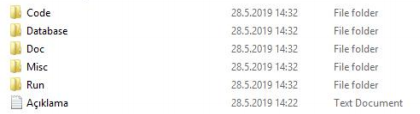
\includegraphics[]{ScreenShot 3.png}
    \caption{Hazırlanacak Dosyalama Şeması}
    \label{fig:fileSchema}
\end{figure}

Proje dosya isimlendirmelerinde iki kişilik projeler için \textbf{OgrNo1\_OgrNo2.rar} olarak grubun öğrenci numaralarının yazılması yeterlidir. Proje dökümanlarına konulması gereken dosyalara ait açıklamalar aşağıda belirtilmiştir. Ayrıca güncelemeler için proje koordinatörlük sayfasını takip etmeniz gerekmektedir. Dosya boyutu, kullanılan veri seti nedeniyle ayrılan alandan fazla olma durumunda, öğrencilerin danışman hocası ile iletişime geçmeleri ve sisteme kullanılan veri seti olmadan proje dökümanları yüklenmelidir.

\begin{itemize}
\item \textbf{Proje Açıklama Dosyası:} \texttt{Açıklama.txt} isminde projenin yeni bir bilgisayara kurulması aşamasında yapılması gereken işlemlerin adım adım anlatıldığı, gerekli ayarlamaların açıklandığı bir dosya hazırlanacaktır. Bu dosyada yazılanların takip edilerek yapılması durumunda projenin çalıştırılabilir olması esastır.

\item \textbf{Proje Kitabı:} \texttt{Doc} klasörü altında projenin basılı olarak teslim edilen kitabının elektronik kopyası yer almalıdır. Diğer bir deyişle kitap hazırlanırken kullanılan \latex dokümanları ve bu dokümanlardan üretilen PDF dosyası yer almalıdır. 

Bilgisayar Projesi öğrencileri için hazırlamaları gereken bildiri formatında 4 sayfalık ingilizce raporun da PDF ve \latex dosyaları yüklenen dökümanlar içeriğinde yer almalıdır.

\item \textbf{Proje Kaynak Kodu:} \texttt{Code} klasörü altında proje dahilinde geliştirilen programların açık kaynak kodları yer almalıdır.

\item \textbf{Projenin Çalıştırılabilir Hali:} \texttt{Run} klasörü altında projenin derlenmiş ve çalıştırmaya hazır şekli yer almalıdır. Özellikle kurularak çalıştırılması gereken uygulamalarda bu dizin altında programın kurulmasını sağlayacak yazılımların (install scripts vb.) listesi .txt dosyası şeklinde belirtilmelidir.

\item \textbf{Proje Veri Tabanı:} \texttt{Database} klasörü altında (var ise) proje içinde kullanılan veritabanının yaratılmasını sağlayan dosyalar (creation scripts) ve veri tabanının proje esnasında kullanılan (içinde örnek bilgilerin bulunduğu) halinin yedeklenmiş hali (backup veya export olarak) bulunmalıdır. Veritabanı kullanlmayan projelerde veri saklanan dosyalar (XML vb.) da bu klasörde yer alabilir. Akademik içerikli projelerde kullanılan veri kümeleri bu klasörde verilebilir. Yüksek boyutlu (>50 MB) veri setlerinde ise, veriye ait kaynak linkinin belirtilmesi yeterlidir.

\item \textbf{Proje içinde kullanılan diğer ek yazılımlar:} \texttt{Misc} klasörü altında proje içinde kullanılan freeware, shareware türü programlar varsa bunlara ait liste .txt olarak belirtilmelidir. (Kullanılan programlama dili, veri tabanı yönetim sistemi, işletim sistemleri gibi yazılımlar buraya kopyalanmamalıdır.)
\end{itemize}
